\question[3]
Zeichne den shortest-path Baum der Breitensuche. Wir beginnen bei a und nehmen an,
dass Knoten auf der gleichen Ebene in alphabetischer Reihenfolge besucht werden.

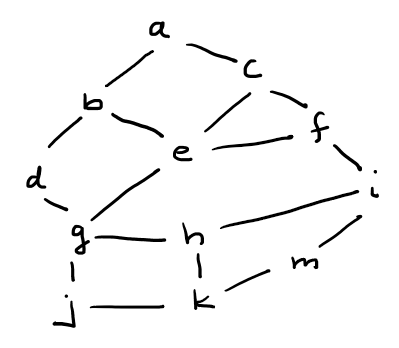
\includegraphics[height=4cm]{\pfad/Graphen/Aufgaben/breitensuche_02/breitensuche_02.png}
\begin{solutionbox}{5cm}
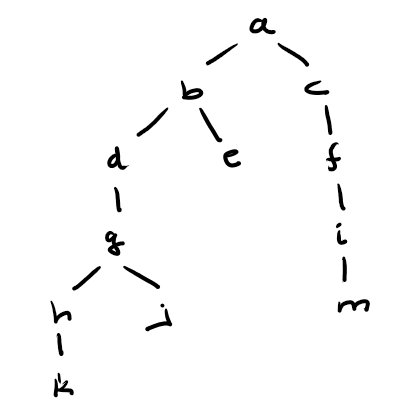
\includegraphics[height=4cm]{\pfad/Graphen/Aufgaben/breitensuche_02/breitensuche_baum_02.png}
\end{solutionbox}
